%% ----------------------------------------------------------------------
%% START OF FILE
%% ----------------------------------------------------------------------

\chapter{关键技术}
\label{cha:key_tech}

\section{IO捕获}
\label{sec:capture_io}

\section{缓存页面替换算法}
\label{sec:cache_algorithm}

当缓存的空间已经满了,又需要有新的数据加入时,就需要使用Cache替换算法释放一定空间以容纳新的缓存块。常用的Cache替换算法可分为三类。本缓存系统对这三种替换算法都进行了实现,使用时可选择任意一种。
\begin{enumerate}

\item 基于访问时间的LRU(Least Recently Used)系列替换算法

LRU替换算法依据缓存块最近一次的访问时间进行决策。当Cache满时,替换出最近最不使用的缓存块。
LRU系列算法实现简单,能够很好的适应数据访问的变化。缺点是没有考虑数据的长期访问特性。最近使用的缓存块可能并不会被经常访问,从而可能导致更需要留在混存中的数据块被替换了出去。

\item 基于使用频度的LFU(Least Frequently Used)系列替换算法

LFU算法依据每个缓存块的访问频度进行决策。当Cache满时,根据替换出历史访问频率最低的缓存块。
LFU算法需要为每个缓存块设置一个计数器,记录访问次数。缺点是需要一定策略对计数器进行清零,否则计数器只增不减会导致某些曾经被频繁访问的缓存块无法及时地被清理出去。

\item 综合时间和频度的替换算法

在决定被替换的缓存块时,只考虑最后一次的访问时间或使用频度都会存在特定的缺陷。论文提出了一种综合考虑访问时间或使用频度的替换算法,经测试,优于LRU和LFU系列算法。
\begin{itemize}
\item
替换算法使用冷、热两个链表管理缓存块(图\ref{fig:replace-algo-1}),初始状态下两个链表均为空。两个链表所能管理的空间之和代表了混存的总容量。
\begin{figure}[htb]
\centering
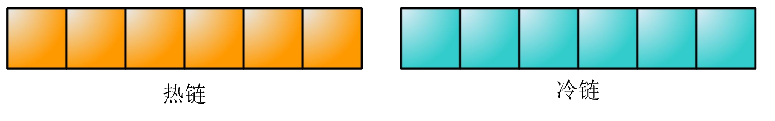
\includegraphics[width=0.6\linewidth]{./graph/replace-algo-1}
\caption{替换算法使用两个链表管理缓存块}
\label{fig:replace-algo-1}
\end{figure}

\item
当冷链表不为满时,新到来的缓存块首先会被加入到冷链表的热端,在运行过程中会统计每个缓存块访问的次数。图\ref{fig:replace-algo-2}展示了缓存块以A->B->C->D->E的字母表顺序加入后的缓存的组织状态状态。
\begin{figure}[htb]
\centering
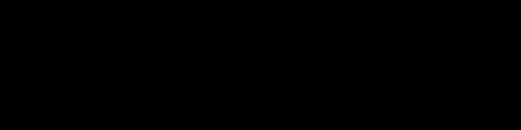
\includegraphics[width=0.6\linewidth]{./graph/replace-algo-2}
\caption{新到来的缓存块加入到冷链表}
\label{fig:replace-algo-2}
\end{figure}

\item
随着系统运行,缓存块会被不断加入。当冷链表已满,而又需要加入新的缓存块时。新的缓存块仍旧会被加入到冷链的热端,为腾出空间冷端就需要移出一个缓存块到临时空间。缓存算法会判断被移出缓存块的引用计数,如果其引用计数大于等于2,则清零其引用计数,并加入到热链表的热端;否则改缓存块占用的空间将会被释放。图\ref{fig:replace-algo-3}展示了加入块G移出块A的过程。
\begin{figure}[htb]
\centering
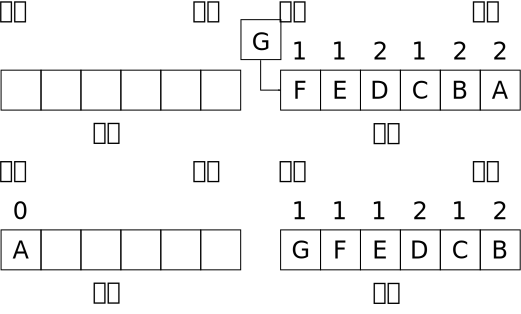
\includegraphics[width=0.6\linewidth]{./graph/replace-algo-3}
\caption{冷链表满时加入缓存块的处理策略}
\label{fig:replace-algo-3}
\end{figure}

\item
新缓存块的持续到来导致冷链表中的缓存块不断被移动到热链表,热链表也会逐渐变满。继续从冷链表向热链表移动缓存块会导致热链表的冷端的缓存块像图\ref{fig:replace-algo-3}中冷链表的冷端的缓存块一样被换出。这些被换出的缓存块的引用计数被清零后,被加入到冷链的热端,重复图\ref{fig:replace-algo-3}的过程。这一过程在图\ref{fig:replace-algo-4}中被描述。
\begin{figure}[htb]
\centering
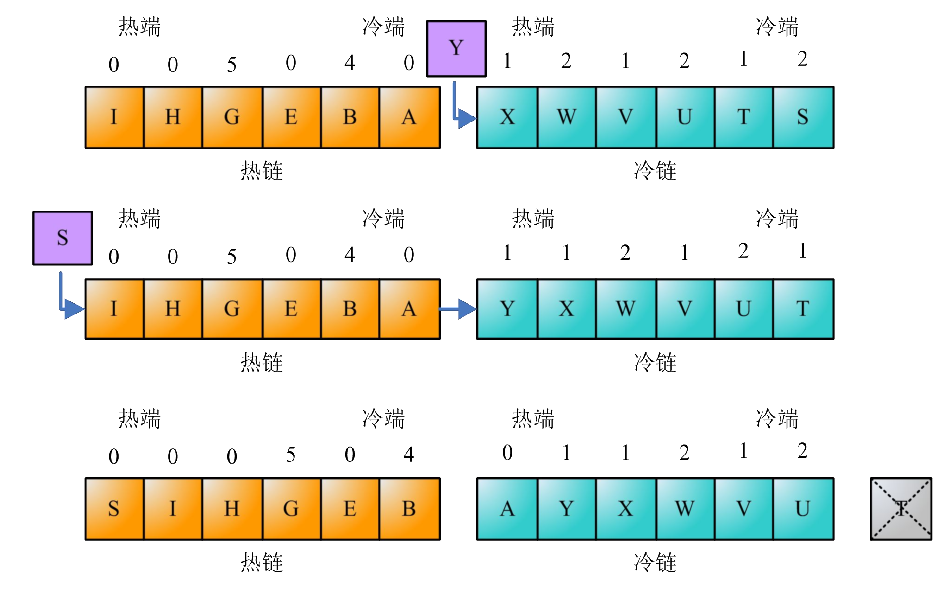
\includegraphics[width=0.7\linewidth]{./graph/replace-algo-4}
\caption{冷热链表均满时加入缓存块的处理策略}
\label{fig:replace-algo-4}
\end{figure}
\end{itemize}

\end{enumerate}

\section{缓存映射策略}
\label{sec:cache_mapping}

存在三种使用最为广泛的缓存映射策略。

\begin{enumerate}

\item 直接相联映射
\\主存储器中的每一块映射到缓存中的某个特定存储块中。缓存中的每个缓存块与主存中的一个或多个存储块相关联(图\ref{fig:cache-map-1})。

\begin{figure}[htb]
\centering
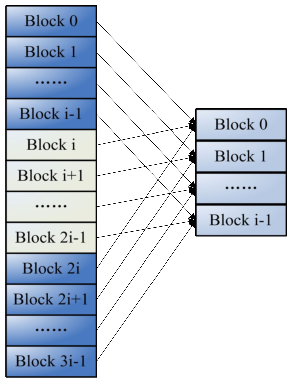
\includegraphics[width=0.3\linewidth]{./graph/cache-map-1}
\caption{直接相联映射}
\label{fig:cache-map-1}
\end{figure}

映射规则:
\begin{itemize}
\item 主存与缓存按照相同大小的数据块组织。
\item 主存容量应是缓存容量的整数倍。将主存空间按缓存的容量分成区,主存中每一区内的块数与缓存的总块数相等。 
\item 主存中某区的一块存入缓存时只能存入缓存中块号相同的位置。
\end{itemize}
设主存的第块i映射到缓存的第j块,则i和j满足如下关系。
j = i mod m	(m为主存每一区的总块数)
直接映射方式的优点是实现简单,可以使用主存地址直接计算出对应的缓存地址,不存在查找过程。缺点是缓存中的每个存储块通常对应主存中多个固定的存储块,运行中如果存在多个块同时被访问会产生缓存替换策略被频繁调用的情况。因此,直接映射适合混存容量为主存的30\%以上时采用,一般应用于超大型系统。

\item 全相联映射
\\主存储器中的任意一块可以映射到缓存中的任意一块(图\ref{fig:cache-map-2})。

\begin{figure}[htb]
\centering
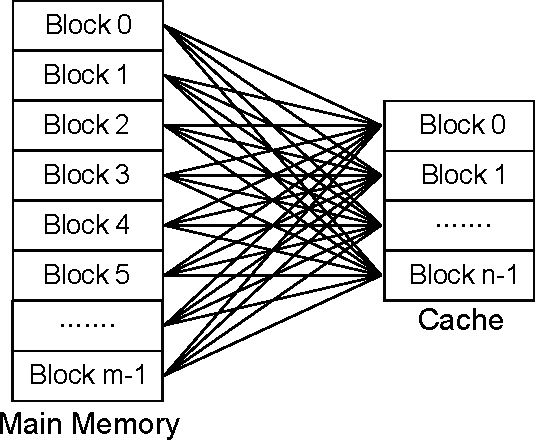
\includegraphics[width=0.3\linewidth]{./graph/cache-map-2}
\caption{全相联映射}
\label{fig:cache-map-2}
\end{figure}

映射规则:
\begin{itemize}
\item 主存与缓存按照相同大小的数据块组织。
\item 主存的某一数据块可以装入缓存的任意一块空间中。
当缓存块数为Cb,主存块数为Mb时,存在Cb×Mb种映射关系。
\end{itemize}
全相联映射的优点是主存和缓存的容量没有限制,只需按照相同大小的数据块进行组织。缺点是当查询主存中的某个数据块是否被缓存时,在不使用额外存储空间的情况下要遍历所有缓存块进行查找。为提高查找效率,可使用多种查找数据结构进行索引,但需要额外的存储空间。

\item 组相联映射
\\主储存器的每一组都与缓存中的某一组相对应,组内的每个块与缓存组内的任意一个存储块相映射(图\ref{fig:cache-map-3})。

\begin{figure}[htb]
\centering
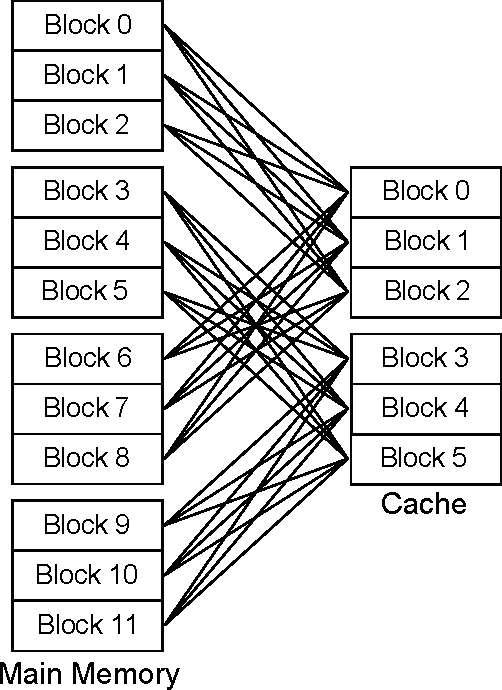
\includegraphics[width=0.4\linewidth]{./graph/cache-map-3}
\caption{组相联映射}
\label{fig:cache-map-3}
\end{figure}

映射规则:
\begin{itemize}
\item 主存与缓存按照相同大小的数据块组织。
\item 主存与缓存以同样的大小划分成组。
\item 主存容量是缓存容量的整数倍,将主存空间按缓存的容量分成区,主存中每一区内的块数与缓存的总块数相等。
\end{itemize}
当主存的数据转储到缓存中时,可以使用主存地址求出唯一对应的缓存组号,也就是主存组内的某一块只能存入同组号的缓存空间内。相关联的两组内各存储块之间则可以任意存放。从主存组到缓存组之间采用直接映射相联方式;在两个对应的组内采用全映射相联方式。

\end{enumerate}

一般从三个方面对不同的映射方式进行比较。
\begin{itemize}
\item 索引速度:直接映射可以直接计算出缓存地址,不需要查找,速度最快;组相联方式则需要查找对应的缓存组,速度次之;全映射的速度最慢。
\item
缓存利用率:全相联映射缓存块的映射是任意的,利用率最高;组相联方式组内映射任意,但是组间相互独立,利用率次之;直接映射缓存中的每个缓存块与主存中的一个或多个存储块相关联,利用率最低。
\item
实现难度:直接映射方式最简单,适合硬件实现;组相联方式和全映射方式的实现难度取决于使用的索引数据结构。当组内块数量较少时组相联方式可以使用遍历的方法,实现相对简单。
\end{itemize}

\section{缓存索引结构}
\label{sec:cache_indexing}

\section{回写策略}
\label{sec:wb_strategy}

对于应用程序的读请求,HDD上的数据不会被改变,因此不存在数据一致性的问题。对于应用程序的写请求,需要决定是直接应用写操作到HDD还是延迟写。学术上存在三种回写策略:写穿法、写回法和写一次法。本系统实现了前两套处理方案。

\subsection{写穿法(Write Through)}
\begin{figure}[htb]
\centering
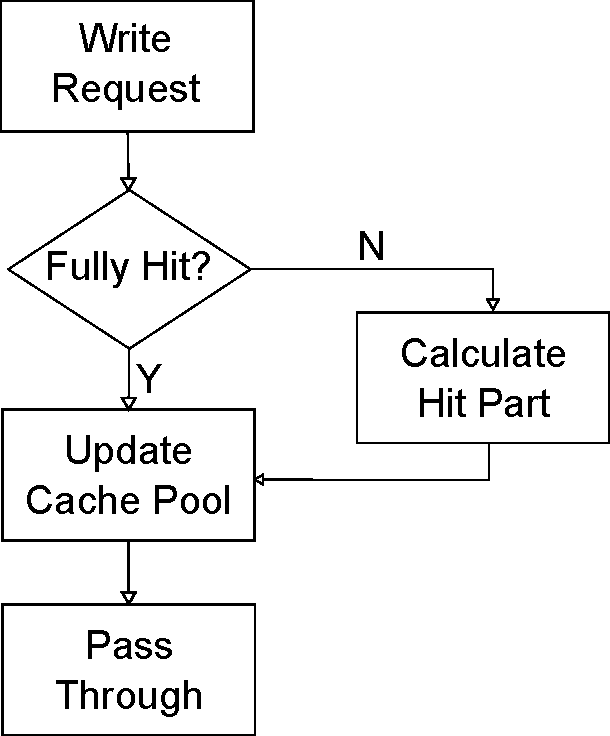
\includegraphics[width=0.4\linewidth]{./graph/write-through}
\caption{写穿法处理策略}
\label{fig:write-through}
\end{figure}

对于写请求,同时应用于HDD和SSD缓存。由于HDD和缓存是同时写入的,因此无需考虑数据一致性问题,也无需为每个缓存块设置标志位标记反映此块是否被修改过(图\ref{fig:write-through})。

\subsection{写回法(Write Back)}
\begin{figure}[htb]
\centering
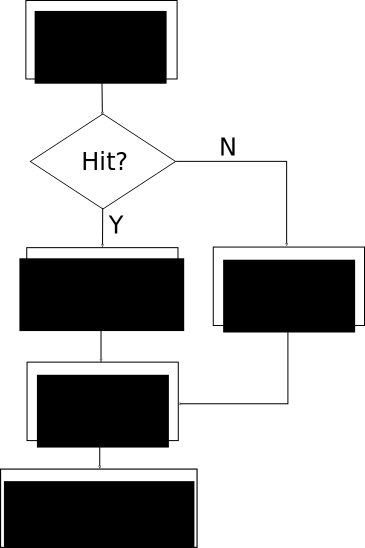
\includegraphics[width=0.4\linewidth]{./graph/write-back}
\caption{写回法处理策略}
\label{fig:write-back}
\end{figure}

对于写请求,在应用于SSD缓存后就结束请求。为每个缓存块设置修改标志,将标志为脏的缓存块加入回写队列(图\ref{fig:write-back-queue})。

\begin{figure}[htb]
\centering
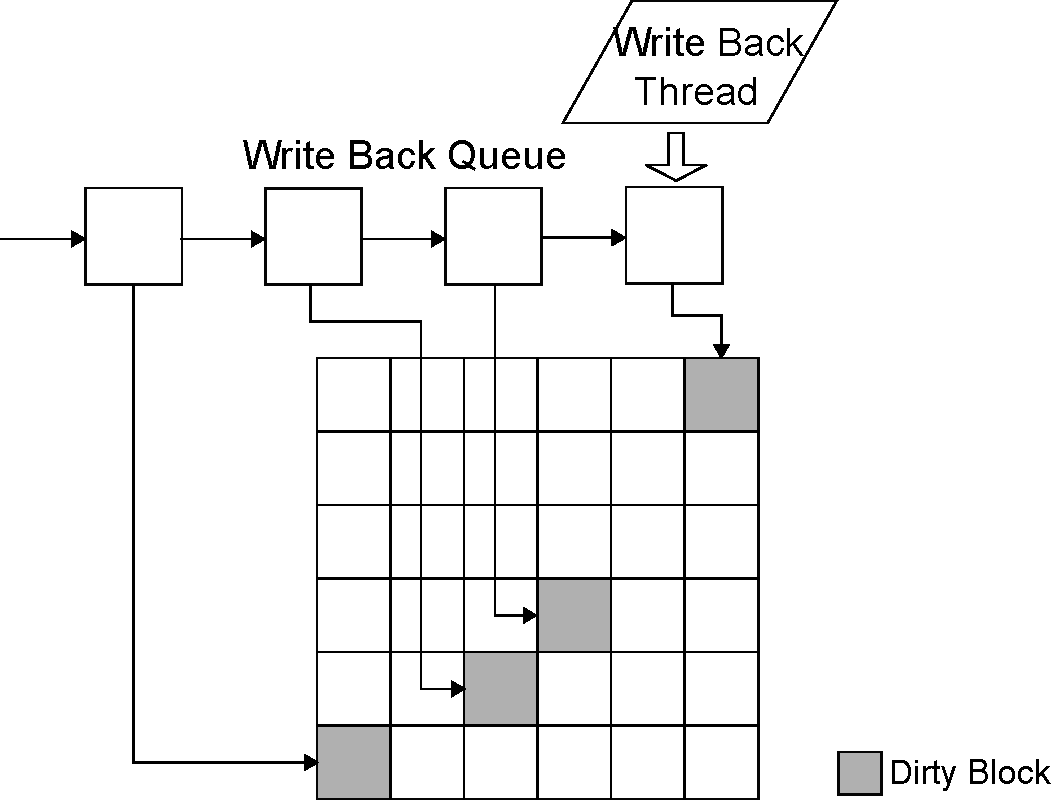
\includegraphics[width=0.4\linewidth]{./graph/write-back-queue}
\caption{指向脏数据块的回写队列}
\label{fig:write-back-queue}
\end{figure}

回写队列的大小是固定。随着脏数据块的加入,当回写队列满时,会触发回写线程进行回写操作。会写线程会将队列中的所有脏缓存块刷回HDD。同样的,当线程接收到回写所有或线程终止信号时,也会进行刷回所有脏缓存块到HDD的操作(图\ref{fig:write-back-thread})。

\begin{figure}[htb]
\centering
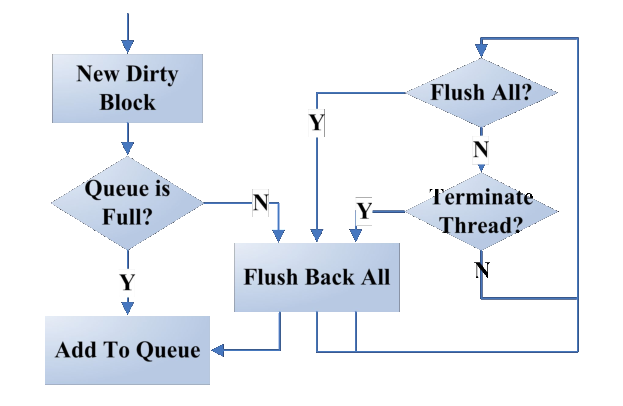
\includegraphics[width=0.6\linewidth]{./graph/write-back-thread}
\caption{回写线程的回写逻辑}
\label{fig:write-back-thread}
\end{figure}

%% ----------------------------------------------------------------------
%%% END OF FILE
%% ----------------------------------------------------------------------